%% ======================================================================
%% 09_validation.tex -- 8. Validacion y caracterizacion (+ validacion del modelo)
%% ======================================================================
\section{Validación y caracterización}
\label{sec:validation}

La validación sigue los escenarios de la guía del curso: movimiento de la base en llano y en una pendiente de \SI{10}{\degree}, equilibrio de la bola con la base fija y en movimiento, y estabilidad de la etapa intermedia (el octocóptero). Todos los resultados provienen de registros tomados el 17, 18, 20 y 23 de noviembre de 2026 y publicados en el repositorio. El error de la bola es la distancia euclidiana entre la bola y el centro del plato (referencia $(0,0)$), calculada solo mientras el PID estaba activo y la bola era detectada.

\subsection{Metodología de ensayos y métricas}
\label{sec:metodologia}
El protocolo de ensayos finales (23/11) definió configuraciones que agregan \emph{un solo elemento a la vez}, para atribuir cada aumento de error a lo que se agregó:
\begin{itemize}
  \item C0: mediciones sin energía (\emph{ejecutada});
  \item C1: \textit{ball and plate} solo, con la base quieta y el dron apagado (\emph{ejecutada});
  \item C2: base en movimiento con el dron trabado a la base, equivalente a la solución \emph{solo servos} (\emph{pendiente});
  \item C3: robot completo con el dron libre en la rótula (\emph{ejecutada}).
\end{itemize}
El protocolo incluye también el ensayo D (comparar C2 y C3 en el mismo ciclo de rampa como prueba directa de la Sección~\ref{sec:porquedron}), así como ensayos específicos de traslación/giro con cinta (E1), barrido sinusoidal del plato (E2), recuperación desde 2 y \SI{5}{\centi\metre} (E3) y descarga de peso $f=0.5$; esas pruebas no se ejecutaron en la campaña del 23/11 y quedan como trabajo futuro (Sección~\ref{sec:limits}). Las métricas definidas en el script \texttt{metricas\_pruebas.py} y su estado de medición se resumen en la Tabla~\ref{tab:metricas}.

\begin{table}[!htbp]
\centering
\small
\caption{Métricas de desempeño, criterios de aceptación y estado de validación. $e(t)$ es la distancia de la bola al centro, en mm, mientras el PID está activo; $R_u=\SI{96.5}{\milli\metre}$ es el radio útil del plato.}
\label{tab:metricas}
\begin{tabularx}{\textwidth}{@{}>{\raggedright\arraybackslash}p{0.23\textwidth}>{\raggedright\arraybackslash}X>{\raggedright\arraybackslash}p{0.22\textwidth}>{\raggedright\arraybackslash}p{0.15\textwidth}@{}}
\toprule
Métrica & Definición & Criterio & Estado \\
\midrule
Error relativo & $e_{\mathrm{RMS}}/R_u\times100$ & E3: $\le\SI{10}{\percent}$ (apagado), $\le\SI{30}{\percent}$ (ralentí); E4/E5: $\le\SI{45}{\percent}$ & medido (Tab.~\ref{tab:ensayos23}) \\
Efectividad & \% del tiempo con $e\le\SI{30}{\milli\metre}$ (y banda de \SI{50}{\milli\metre} en 23/11) & E3: $\ge\SI{90}{\percent}$; E4/E5: $\ge\SI{60}{\percent}$ & medido (Tab.~\ref{tab:ensayos23}--\ref{tab:completos23}) \\
Pérdidas y tasa de éxito & intervalos $>\SI{1}{\second}$ sin bola; ensayos sin pérdida / totales & $\ge\SI{80}{\percent}$ & medido en banco y rampa \\
Recuperación (2 y \SI{5}{\centi\metre}) & tiempo hasta entrar a la banda (5 o \SI{20}{\milli\metre}) y quedarse \SI{2}{\second}; sobrepaso & $\le$3 y \SI{5}{\second}; éxito $\ge\SI{80}{\percent}$ & pendiente (E3) \\
Esfuerzo de control de los servos & $\sqrt{\overline{(u_x-n_x)^2+(u_y-n_y)^2}}$ (\si{\micro\second}); actividad $\sum|\Delta u|/T$ & comparar C1, C2 y C3, y D-A con D-B & C1/C3 medidos; C2 y D pendientes \\
Uso y saturación de los servos & media de $\max|u-n|/\SI{220}{\micro\second}$; \% del tiempo $\ge\SI{95}{\percent}$ & saturación $\le\SI{10}{\percent}$ & medido (18/11 y Pi 23/11) \\
Esfuerzo del dron & dispersión de los 8 motores (\si{\micro\second}) y colectivo medio & cero cortes en modo base & medido (Sec.~\ref{sec:flights}--\ref{sec:ensayos23}) \\
Base: traslación y giro & $|d-d_{\mathrm{ref}}|/d_{\mathrm{ref}}$ y $|\psi-\SI{360}{\degree}|/\SI{360}{\degree}$ & $\le\SI{5}{\percent}$ & velocidad y desvío medidos; 25/50\,cm y \SI{360}{\degree} pendientes \\
Plataforma & frecuencia máxima con amplitud $\ge\SI{70}{\percent}$ (barrido 0,5--\SI{4}{\hertz}) & $\ge\SI{1}{\hertz}$ & pendiente (E2) \\
\bottomrule
\end{tabularx}
\end{table}

\paragraph{Mediciones sin energía (C0, 23/11)} Estas mediciones fijaron los parámetros que el modelo tomaba del CAD o de estimaciones:
\begin{itemize}
  \item la masa total del robot, \SI{10.4}{\kilo\gram};
  \item la distancia entre ejes, \SI{0.22}{\metre};
  \item el recorrido de la guía, unos \SI{140}{\milli\metre} (el CAD indicaba \SI{77}{\milli\metre});
  \item las pendientes de vuelco estático, \SI{21.5}{\degree} y \SI{30.5}{\degree}, de las que salen $x_G=\SI{88}{\milli\metre}$ y $h_G=\SI{224}{\milli\metre}$;
  \item el rango de la rótula: \SI{35}{\degree} hacia M8, \SI{40}{\degree} hacia M6, \SI{47}{\degree} hacia M5 y \SI{53}{\degree} hacia M7.
\end{itemize}
El rango de la rótula supera con holgura los \SI{10}{\degree} que cambia la base en cada quiebre de la rampa. Por tanto, los cortes por inclinación del 18/11 al entrar a la rampa no se debieron a que el módulo chocara con el tope. Se explican por la dinámica: el golpe en el quiebre, sobre un péndulo invertido con poca autoridad de par en ralentí.

\subsection{Octocóptero en banco (rotores en ralentí)}
El 18/11 el dron funcionó con un colectivo fijo de \SI{1300}{\micro\second} sobre la rótula libre mientras se lo empujaba con la mano. El búfer a bordo se registró a 190--\SI{200}{\hertz} (Fig.~\ref{fig:bench}).

\begin{itemize}
  \item En los dos ensayos, el alabeo RMS fue \SI{0.38}{\degree} y \SI{0.26}{\degree}, y el cabeceo RMS, \SI{0.26}{\degree} y \SI{0.24}{\degree}.
  \item La inclinación máxima fue \SI{1.42}{\degree}.
  \item Las órdenes de motor se mantuvieron entre \SI{1255}{\micro\second} y \SI{1338}{\micro\second}, es decir, con poco esfuerzo de control.
  \item Tras el mayor empujón (\SI{3.7}{\degree}), el dron volvió a nivelarse en alrededor de \SI{1}{\second}.
\end{itemize}

\begin{figure}[!htbp]
  \centering
  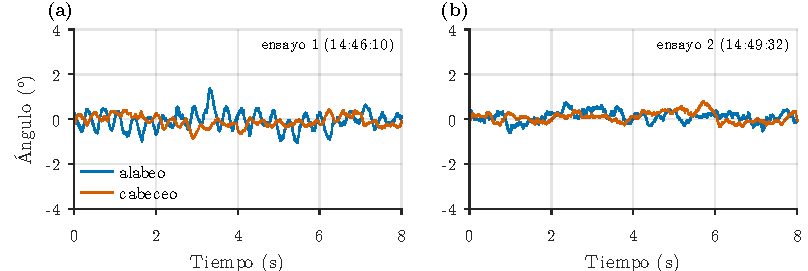
\includegraphics{figures/fig_drone_bench.pdf}
  \caption{Actitud del octocóptero sobre la rótula libre con colectivo de ralentí (\SI{1300}{\micro\second}), registro a bordo a 190--\SI{200}{\hertz}.}
  \label{fig:bench}
\end{figure}

\subsection{Campaña de vuelo en la guía}
\label{sec:flights}
El 20/11 se hicieron nueve vuelos en la guía con versiones sucesivas del firmware, con las LiPo cargadas a 12,4\,V en reposo al iniciar la sesión de la tarde. La Tabla~\ref{tab:flights} y la Fig.~\ref{fig:flights} los resumen.

\begin{itemize}
  \item \textbf{Vuelos 1--2.} Revelaron dos problemas: la saturación del acelerómetro por la vibración de los rotores (\SIrange{0.03}{2.2}{g}), que producía un falso corte por inclinación, y un giro real de guiñada del dron sobre la rótula. De ahí salieron el filtro de \SI{10}{\hertz} del acelerómetro y el lazo de guiñada.
  \item \textbf{Vuelos 3--6.} Despegaron, pero derivaron lentamente en cabeceo o alabeo hasta que el operador o el enclavamiento los detuvo. La deriva tenía un periodo de 5--\SI{10}{\second} y era la misma con ganancias completas (v5) y reducidas (v6). Esto apuntaba al límite de autoridad de par de la Sección~\ref{sec:authority}, cuya región de atracción era de solo 3--4$^\circ$, y no a las ganancias.
  \item \textbf{Vuelo 7} (v8, límite de velocidad angular más amplio). Primer vuelo estacionario estable: \SI{20}{\second} a 1725--\SI{1775}{\micro\second}, con alabeo RMS de \SI{0.55}{\degree} y cabeceo RMS de \SI{1.19}{\degree}. Se cortó durante el aterrizaje, cuando las ganancias volvieron a los valores de banco con el dron aún en el aire.
  \item \textbf{Vuelos 8--9} (v9, con histéresis). Volaron y aterrizaron sin corte. En el vuelo 9 el despegue necesitó \SI{1796}{\micro\second}, \SI{21}{\micro\second} más que en el vuelo 8, y el colectivo se subió hasta \SI{1816}{\micro\second}; tras \SI{48}{\second} de vuelo estacionario el cabeceo divergió hasta el límite de \SI{12}{\degree}. La saturación de la asignación no lo explica, porque \eqref{eq:taumax} aún da \SI{2.4}{\newton\metre}. Los candidatos son el modo lento poco amortiguado de la Sección~\ref{sec:attitude}, cuyo amortiguamiento depende de $k_T$, y la caída de tensión de la batería, que reduce $k_T$ con $V_{\mathrm{bus}}^2$: al final del vuelo 9 las LiPo habían entregado \SI{1.0}{\ampere\hour} cada una en la tarde (Sección~\ref{sec:bateria}). Más tarde, con 11,1\,V, el módulo ya no despegó.
\end{itemize}

\begin{table}[!htbp]
\centering
\caption{Campaña de vuelo en la guía (20/11/2026). Error RMS respecto a la horizontal, calculado mientras la orden media de motor superaba \SI{1650}{\micro\second}.}
\label{tab:flights}
\footnotesize
\setlength{\tabcolsep}{4pt}
\begin{tabularx}{\textwidth}{@{}clrrrrr>{\raggedright\arraybackslash}X@{}}
\toprule
Vuelo & FW & Col.\ máx. & $t$ & Alabeo & Cabeceo & Incl. & Resultado \\
 & & (\si{\micro\second}) & (\si{\second}) & RMS (°) & RMS (°) & máx.\ (°) & \\
\midrule
1 & v2 & 1625 & 0 & -- & -- & -- & corte por inclinación (vibración en el acelerómetro) \\
2 & v3 & 1475 & 0 & -- & -- & -- & corte por guiñada ($-20^\circ$) \\
3 & v4 & 1700 & 10,9 & 0,93 & 4,89 & 9,8 & parada del operador, deriva en cabeceo \\
4 & v5 & 1800 & 19,4 & 2,99 & 0,95 & 9,3 & parada del operador, oscilación lenta \\
5 & v6 & 1700 & 3,1 & 0,83 & 3,59 & 10,9 & corte por inclinación al despegar \\
6 & v6 & 1725 & 8,4 & 4,14 & 1,38 & 11,1 & corte por alabeo (videos IMG\_1867--1868) \\
7 & v8 & 1775 & 27,2 & 0,55 & 1,19 & 4,3 & estacionario \SI{20}{\second}; corte al aterrizar (video IMG\_1869) \\
8 & v9 & 1775 & 31,0 & 1,15 & 0,95 & 3,8 & estacionario y aterrizaje, sin corte \\
9 & v9 & 1816 & 62,0 & 1,73 & 1,70 & 10,8 & estacionario \SI{48}{\second}; corte por cabeceo \\
\bottomrule
\end{tabularx}
\end{table}

\begin{figure}[!htbp]
  \centering
  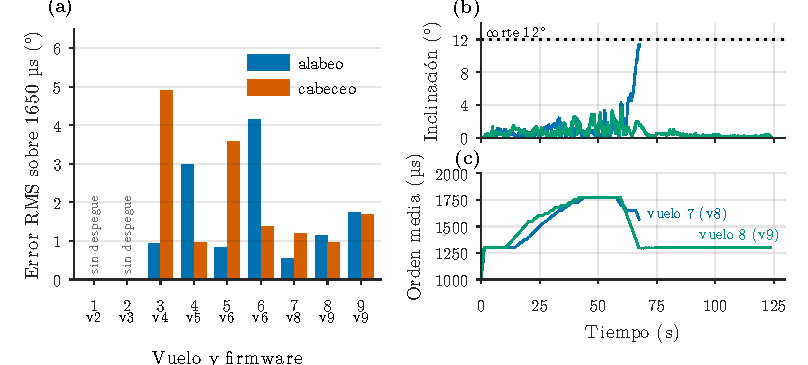
\includegraphics{figures/fig_flight_campaign.pdf}
  \caption{Campaña de vuelo en la guía. (a) Error RMS de alabeo y cabeceo por encima de \SI{1650}{\micro\second} en cada vuelo, con su versión de firmware. (b) Inclinación y (c) orden media de motor de los vuelos 7 (v8) y 8 (v9): el v8 se corta cuando las ganancias de vuelo se desactivan durante el aterrizaje, y el v9 aterriza con normalidad.}
  \label{fig:flights}
\end{figure}

\paragraph{Videos sincronizados con la telemetría}
Los tres videos del 20/11 (iPhone, 4K a \SI{120}{fps}) se sincronizaron con los registros por la hora de creación del archivo, que en el iPhone marca el inicio de la grabación, y por la hora del PC en cada línea del registro (Fig.~\ref{fig:video}). IMG\_1867 (15:10:11, \SI{11}{\second}) muestra el vuelo 6 mientras el colectivo sube de 1600 a \SI{1675}{\micro\second}. IMG\_1868 (15:10:26, \SI{4}{\second}) muestra su final: el alabeo pasa de $-6^\circ$ a $-11{,}1^\circ$ en \SI{1.3}{\second}, el firmware corta los motores y el módulo cae sobre la guía, lo que coincide con el registro con un desfase menor que \SI{1}{\second}. IMG\_1869 (15:23:32, \SI{13}{\second}) cae dentro del vuelo estacionario del vuelo 7, con el colectivo entre 1763 y \SI{1775}{\micro\second} y la inclinación entre 0,1 y 1,7$^\circ$. En los tres videos un operador acompaña con la mano el mástil de la cámara como medida de seguridad; el video no permite descartar un apoyo leve, que actuaría como una perturbación más sobre el lazo de actitud; las cifras de la Tabla~\ref{tab:flights} se toman tal como salen del registro.

\begin{figure}[!htbp]
  \centering
  \begin{subfigure}[b]{0.24\textwidth}\centering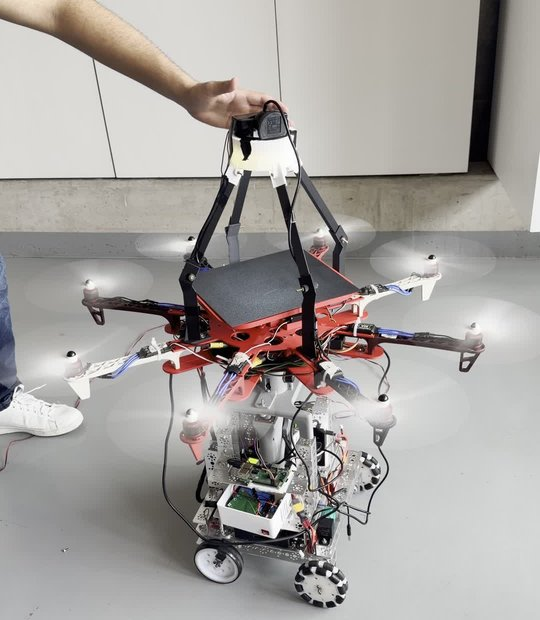
\includegraphics[width=\linewidth]{figures/video_a.jpg}\caption{Vuelo 6, \SI{1650}{\micro\second}.}\end{subfigure}\hfill
  \begin{subfigure}[b]{0.24\textwidth}\centering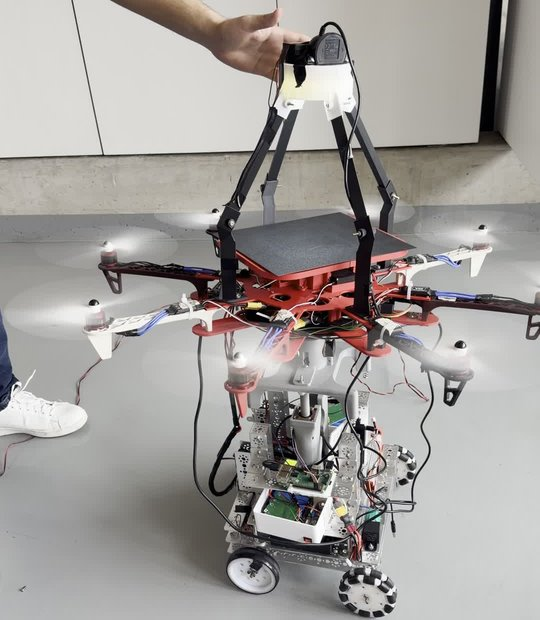
\includegraphics[width=\linewidth]{figures/video_b.jpg}\caption{Vuelo 6, \SI{1724}{\micro\second}.}\end{subfigure}\hfill
  \begin{subfigure}[b]{0.24\textwidth}\centering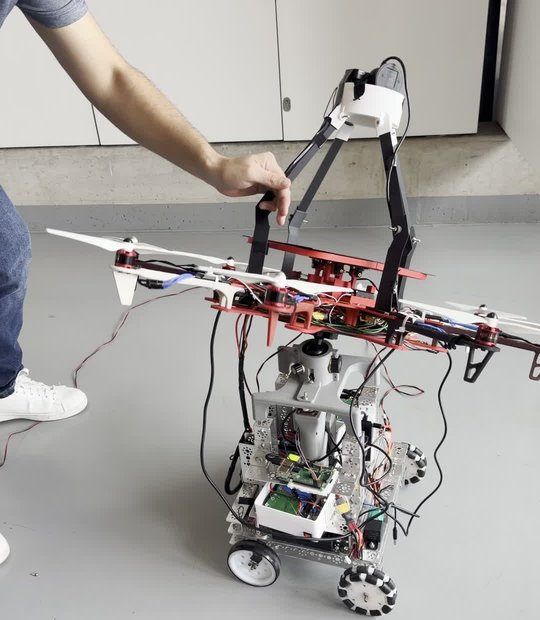
\includegraphics[width=\linewidth]{figures/video_c.jpg}\caption{Vuelo 6, tras el corte.}\end{subfigure}\hfill
  \begin{subfigure}[b]{0.24\textwidth}\centering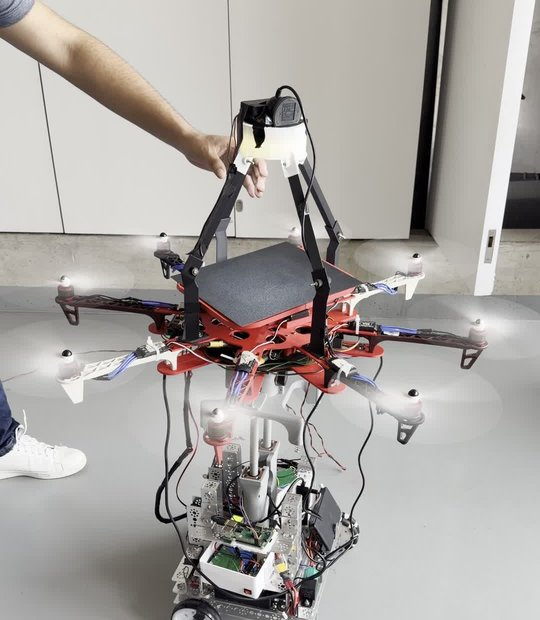
\includegraphics[width=\linewidth]{figures/video_d.jpg}\caption{Vuelo 7, \SI{1774}{\micro\second}.}\end{subfigure}
  \caption{Cuadros de los videos del 20/11 sincronizados con la telemetría: (a) IMG\_1867 a los \SI{6}{\second}, (b) IMG\_1868 a \SI{1}{\second}, (c) IMG\_1868 a \SI{3.2}{\second}, después del corte por alabeo de $-11{,}1^\circ$, con los motores detenidos y el módulo apoyado de lado, y (d) IMG\_1869 a los \SI{7}{\second}, en vuelo estacionario con 0,4--0,6$^\circ$ de inclinación. Las LiPo estaban cerca de 12,4\,V.}
  \label{fig:video}
\end{figure}

\paragraph{Comparación con el modelo de Isaac Lab}
Antes de los ensayos, el conjunto se modeló en Isaac Lab \cite{mittal2023} a partir del CAD, con la rótula y la guía (\SI{3.6}{\kilo\gram}, empuje limitado a \SI{6}{\newton} por motor). Allí se entrenaron y evaluaron una política PPO \cite{schulman2017} y un controlador clásico PI-D. La comparación muestra dos resultados distintos:
\begin{itemize}
  \item \textbf{Empuje.} El modelo predijo el vuelo estacionario en \SI{1899}{\micro\second} (\SI{4.41}{\newton} por motor); el conjunto real despegó 124--\SI{174}{\micro\second} antes, es decir, la ganancia real de empuje es 33--52\% mayor (Sección~\ref{sec:ident}). El modelo de empuje era conservador, y ese error, no el diseño del controlador, es lo que puso al lazo de actitud real dentro de la región estable de la Fig.~\ref{fig:dronestab}b. El simulador tampoco modelaba la tensión de la batería, que en el prototipo mueve el despegue más de \SI{100}{\micro\second} entre carga completa y descarga (Sección~\ref{sec:bateria}).
  \item \textbf{Actitud.} La inclinación RMS simulada fue \SI{0.02}{\degree} con PPO, \SI{0.04}{\degree} con el controlador clásico y \SI{0.12}{\degree} con perturbaciones; los valores medidos son 0,55--\SI{1.7}{\degree}. El modelo ignoraba cuatro efectos que dominaron el comportamiento real: la vibración de los rotores en la IMU, la excentricidad del centro de masa (\SI{9.5}{\milli\metre}), la saturación de la orden de velocidad angular, y el retraso y el retardo de actuación que, junto con el polo del péndulo invertido, ponen al lazo cerca del límite de la Sección~\ref{sec:limits_fund}. Los ocho motores simulados eran simétricos, mientras que la dispersión mediana real entre motores fue 50--\SI{90}{\micro\second}.
\end{itemize}

\subsection{\textit{Ball and plate} con la base fija y en movimiento}
La Fig.~\ref{fig:bp} y la Tabla~\ref{tab:bp} comparan cuatro condiciones:
\begin{enumerate}[label=(\alph*)]
  \item base quieta con el dron apagado (17/11, \SI{75}{\second});
  \item base quieta con los ocho rotores en ralentí y el lazo de actitud activo (17/11, \SI{469}{\second});
  \item robot avanzando en recta y girando en llano (18/11, cuatro recorridos, \SI{582}{\second});
  \item robot subiendo y bajando la rampa de \SI{10}{\degree} (18/11, seis recorridos, \SI{345}{\second}).
\end{enumerate}
Cada recorrido de (c) y (d) se emparejó con su video por la marca de tiempo del archivo de video.

\begin{table}[!htbp]
\centering
\caption{Error de la bola $|e|$ (distancia al centro del plato, en mm) en las cuatro condiciones. Diámetro de la bola \SI{27}{\milli\metre}; medio ancho del plato \SI{110}{\milli\metre}.}
\label{tab:bp}
\small
\begin{tabular}{@{}lrrrrr@{}}
\toprule
Condición & Muestras & Mediana & Media & P90 & P95 \\
\midrule
(a) base quieta, dron apagado & 13\,951 & 4,4 & 4,4 & 4,4 & 4,5 \\
(b) base quieta, dron en ralentí & 85\,219 & 18,9 & 23,1 & 39,9 & 60,4 \\
(c) en movimiento, llano & 95\,851 & 27,9 & 33,1 & 63,2 & 76,2 \\
(d) en movimiento, rampa de \SI{10}{\degree} & 62\,492 & 29,5 & 35,8 & 63,9 & 87,9 \\
\bottomrule
\end{tabular}
\end{table}

\begin{figure}[!htbp]
  \centering
  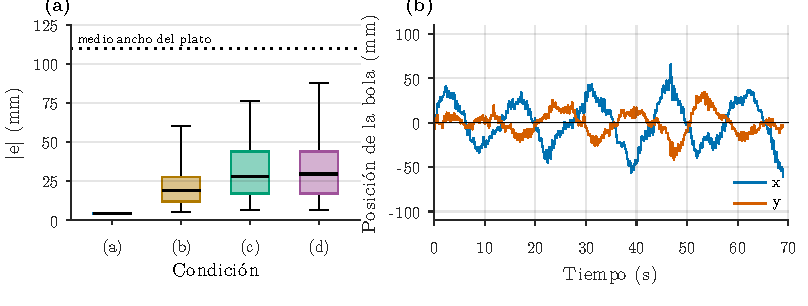
\includegraphics[width=\textwidth]{figures/fig_bp_results.pdf}
  \caption{Izquierda: distribución del error de la bola en las condiciones (a)--(d) de la Tabla~\ref{tab:bp} (caja: cuartiles; bigotes: percentiles 5 y 95). Derecha: posición de la bola durante un recorrido en la rampa (video \texttt{VID\_20261118\_165747}).}
  \label{fig:bp}
\end{figure}

\paragraph{Discusión}
\begin{itemize}
  \item \textbf{Dron apagado.} Con el dron apagado, el error es constante, \SI{4.4}{\milli\metre}: la bola se detiene dentro de la zona muerta de los servos. El ruido de visión está muy por debajo de ese valor.
  \item \textbf{Rotores en ralentí.} Encender los rotores multiplica por cuatro el error mediano (a \SI{18.9}{\milli\metre}). El modelo de propagación muestra que la actitud residual del octocóptero (dentro de \SI{0.4}{\degree}) explica solo unos \SI{2}{\milli\metre} RMS; el resto es una carga lenta que actúa directamente sobre la bola (flujo de los rotores, vibración y juego), concentrada por debajo de \SI{0.3}{\hertz} (Sección~\ref{sec:coupling}). Con las ganancias anteriores ($k_i=0.2$) la bola caía en menos de \SI{5}{\second}; tras subir la ganancia integral a 0,8 no hubo caídas en una prueba de \SI{20}{\second}, y se completó el ensayo de \SI{469}{\second} de la condición (b).
  \item \textbf{Base en movimiento.} Mover la base suma unos \SI{10}{\milli\metre} a la mediana y ensancha la cola (P95 de 76--\SI{88}{\milli\metre}), de acuerdo con el término de aceleración de la rótula de \eqref{eq:balllinx} y su amplificación a través del octocóptero (Fig.~\ref{fig:transm}c). La rampa es solo un poco peor que el llano: como predice \eqref{eq:tilt}, la rótula esférica absorbe la pendiente de \SI{10}{\degree} y el octocóptero mantiene nivelado el plato. Con la bandeja fija a la base, esa misma pendiente habría dejado a los servos con \SI{0.8}{\degree} de recorrido útil (Sección~\ref{sec:porquedron}).
  \item \textbf{Detección de la bola.} En los recorridos con la base en movimiento la bola se detectó el 61--100\% del tiempo. Los huecos incluyen caídas por el borde del plato, a menudo en los bordes de la rampa, donde el acelerómetro registró golpes de hasta \SI{1.95}{g}, y los momentos en que la bola se repuso con la mano.
\end{itemize}

\begin{figure}[!htbp]
  \centering
  \begin{subfigure}[b]{0.32\textwidth}\centering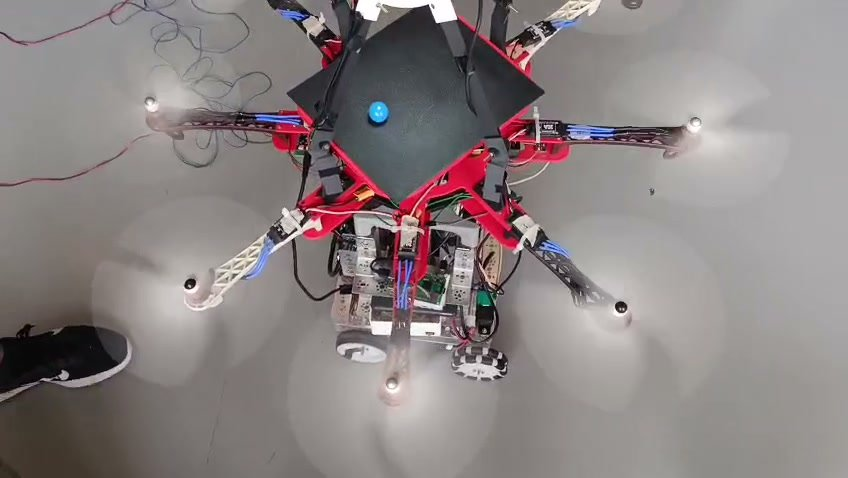
\includegraphics[width=\linewidth]{figures/photo_flat_turn.jpg}\caption{Giro en llano.}\end{subfigure}\hfill
  \begin{subfigure}[b]{0.32\textwidth}\centering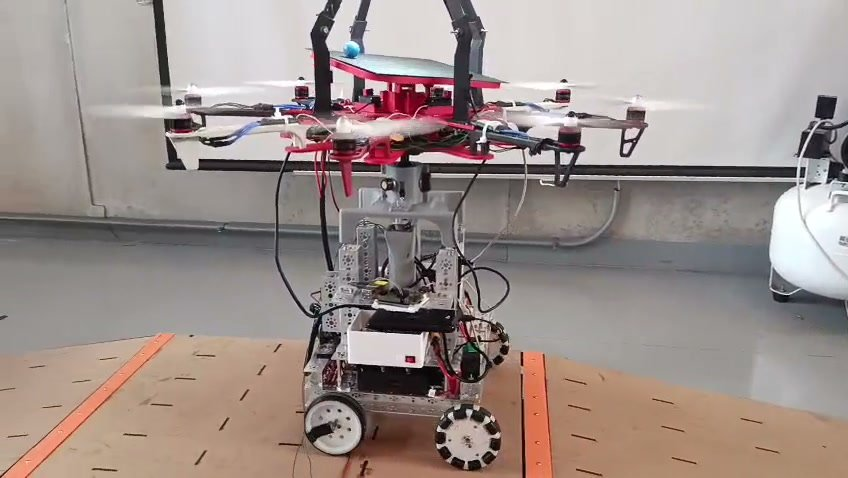
\includegraphics[width=\linewidth]{figures/photo_ramp_climb.jpg}\caption{Subiendo la rampa.}\end{subfigure}\hfill
  \begin{subfigure}[b]{0.32\textwidth}\centering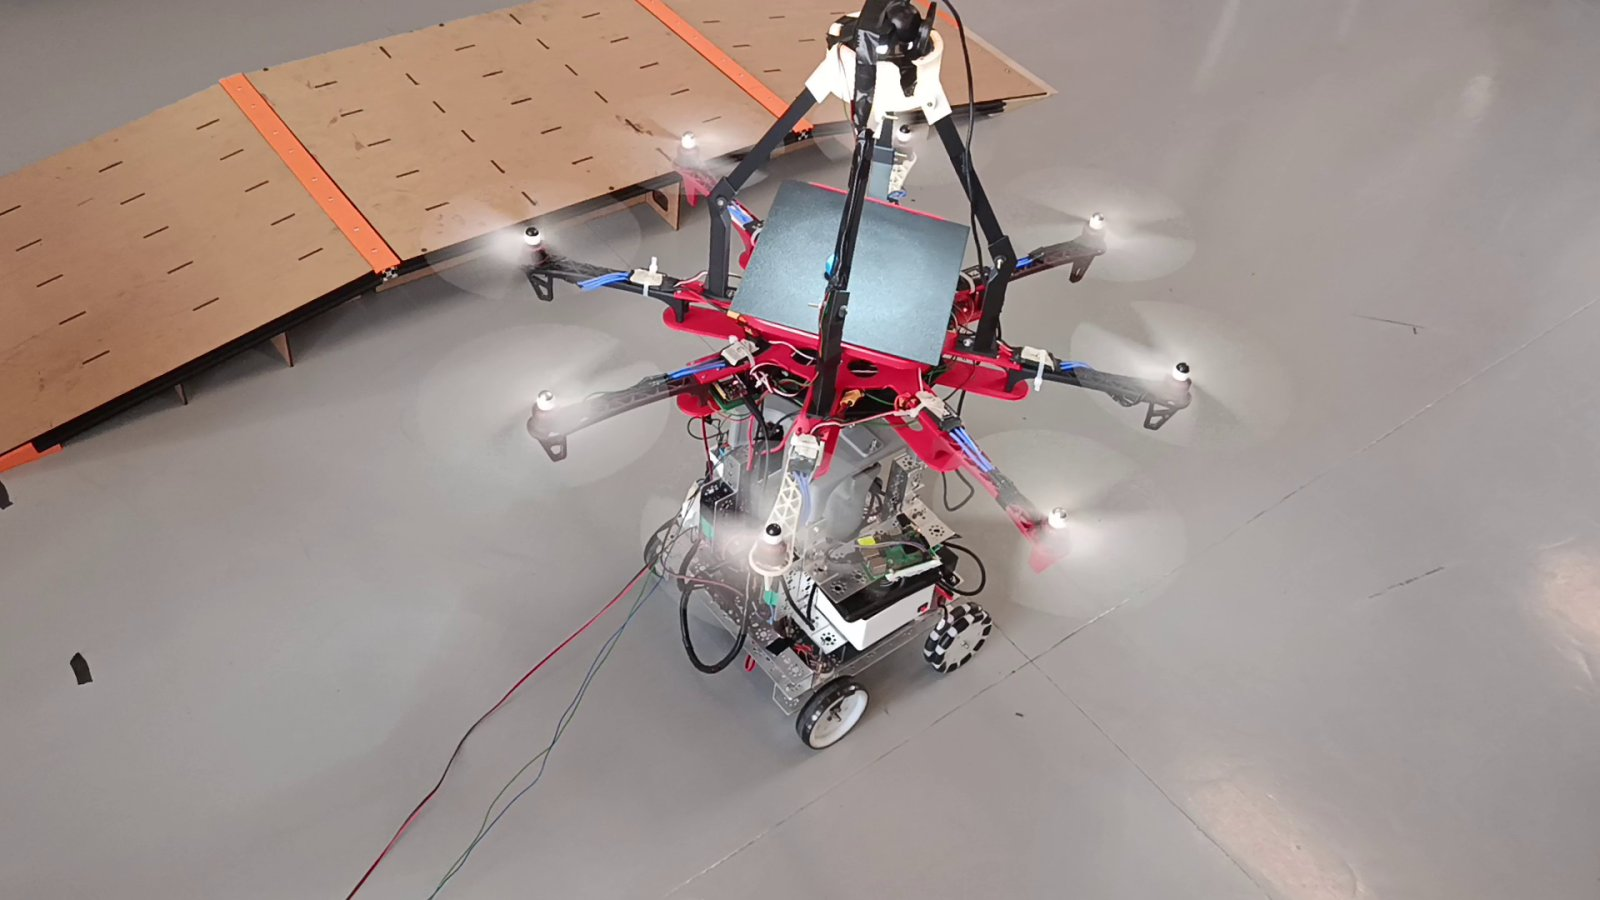
\includegraphics[width=\linewidth,trim=200 0 200 0,clip]{figures/photo_ramp_top.jpg}\caption{En lo alto de la rampa.}\end{subfigure}
  \caption{Pruebas integradas del 18/11/2026 con los rotores girando y la bola sobre el plato (cuadros de los videos de las pruebas).}
  \label{fig:tests}
\end{figure}

\subsection{Ensayos finales del robot completo (23/11)}
\label{sec:ensayos23}
El 23/11 se repitió el equilibrio de la bola sobre el robot completo: la base TETRIX con el octocóptero en la rótula y el \textit{ball and plate} encima, con el firmware v11 del dron (Secciones~\ref{sec:altura} y \ref{sec:metodologia}). Se registraron \textbf{13 ensayos} de equilibrio de entre 23 y \SI{122}{\second}, \SI{816}{\second} en total; en 10 de ellos los ocho rotores estaban encendidos (\SI{614}{\second}). Un ensayo empieza cuando el PID ve la bola dentro del plato y termina cuando la bola sale del plato o el operador lo detiene; se descartan sus primeros \SI{3}{\second}, en los que la bola se coloca a mano. La Tabla~\ref{tab:ensayos23} y la Fig.~\ref{fig:ensayos23} los resumen.

\paragraph{Origen de los datos y verificación} La Raspberry Pi registró la bola a \SI{187}{\hertz} (\texttt{registro\_20261123\_182316.csv}, 18:23--18:39), pero sus registros de antes y después de ese tramo no pudieron descargarse antes del informe. Para esos ensayos se recuperó la telemetría de las dos grabaciones de pantalla de la interfaz web (17:29 y 18:36): la página dibuja en vivo la bola sobre el mapa del plato y la inclinación del dron sobre sus círculos de 2, 5 y \SI{12}{\degree}, y el script \texttt{extraer\_de\_grabacion.py} mide la posición de esos puntos cuadro a cuadro (unos \SI{13}{\hertz}) con las escalas del código de la página. En los tramos que cubren a la vez la grabación y el registro de la Pi, la posición recuperada difiere de la registrada en 0,6 y \SI{1.4}{\milli\metre} de mediana (P90 de \SI{6.4}{\milli\metre}; 4007 muestras), muy por debajo de los errores que se reportan, así que ambas fuentes se tratan juntas. La recuperación no da los pulsos de los servos ni el colectivo del dron, pero sí el estado de la placa y de los motores.

\begin{table}[!htbp]
\centering
\caption{Ensayos de equilibrio de la bola sobre el robot completo (23/11/2026). Rot.: rotores encendidos. Fuente: registro de la Pi a \SI{187}{\hertz} o telemetría recuperada de la grabación de pantalla. Errores en mm; error relativo $e_{\mathrm{RMS}}/R_u$ en \%; efectividad: \% del tiempo con $e\le\SI{50}{\milli\metre}$. $^\ast$: ensayo completo, con la base cruzando la rampa (Tabla~\ref{tab:completos23}).}
\label{tab:ensayos23}
\footnotesize
\setlength{\tabcolsep}{3.5pt}
\begin{tabular}{@{}clrclrrrrrc@{}}
\toprule
Ens. & Hora & $t$ (s) & Rot. & Fuente & Mediana & RMS & P95 & Error rel. & Efect. & $\sigma_x$ / $\sigma_y$ \\
 & & & & & & & & & ($\le$\SI{50}{\milli\metre}) & \\
\midrule
01 & 17:30 & 27,0 & sí & video & 29,2 & 33,7 & 56,2 & 34,9 & 88,5 & 30,9 / 11,1 \\
02 & 17:32 & 98,5 & sí & video & 31,8 & 35,3 & 54,9 & 36,6 & 90,5 & 32,3 / 14,3 \\
03 & 17:45 & 122,3 & no & video & 31,5 & 35,0 & 55,7 & 36,3 & 92,1 & 31,2 / 15,7 \\
04 & 18:25 & 22,9 & no & Pi & 44,0 & 51,9 & 94,0 & 53,8 & 63,3 & 49,3 / 11,8 \\
05 & 18:26 & 95,9 & sí & Pi & 39,2 & 51,0 & 99,2 & 52,9 & 67,9 & 49,2 / 13,4 \\
06 & 18:33 & 57,0 & no & Pi & 31,3 & 45,1 & 97,1 & 46,7 & 77,5 & 41,6 / 14,9 \\
07 & 18:36 & 83,5 & sí & Pi & 33,5 & 38,3 & 63,9 & 39,7 & 81,2 & 35,5 / 14,4 \\
08 & 18:40 & 57,4 & sí & video & 42,8 & 46,1 & 72,8 & 47,7 & 65,4 & 40,8 / 20,9 \\
09 & 18:45 & 60,6 & sí & video & 35,1 & 47,3 & 86,5 & 49,0 & 70,2 & 43,4 / 18,8 \\
10$^\ast$ & 18:49 & 39,1 & sí & video & 33,2 & 41,4 & 67,8 & 42,9 & 71,7 & 38,4 / 12,7 \\
11$^\ast$ & 18:51 & 54,7 & sí & video & 42,0 & 48,0 & 82,9 & 49,7 & 67,1 & 38,3 / 28,1 \\
12$^\ast$ & 18:55 & 45,3 & sí & video & 33,4 & 42,6 & 77,4 & 44,1 & 75,7 & 37,2 / 19,6 \\
13$^\ast$ & 19:00 & 51,5 & sí & video & 33,5 & 41,0 & 73,2 & 42,5 & 77,3 & 38,4 / 14,4 \\
\midrule
\multicolumn{5}{@{}l}{Mediana de los 13 ensayos} & 33,5 & 42,6 & 73,2 & 44,1 & 75,7 & 38,3 / 14,4 \\
\bottomrule
\end{tabular}
\end{table}

\begin{figure}[!htbp]
  \centering
  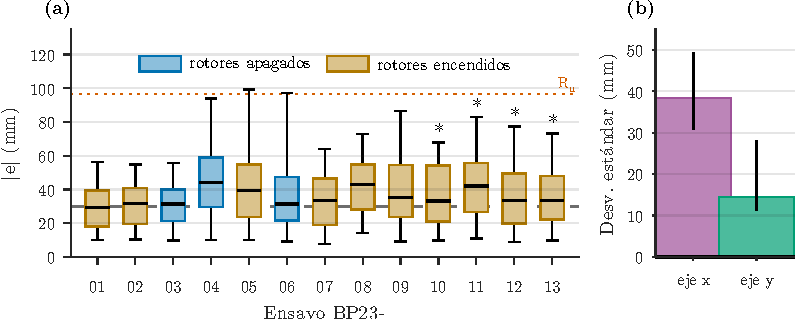
\includegraphics[width=\textwidth]{figures/fig_ensayos_23nov.pdf}
  \caption{Ensayos del 23/11 sobre el robot completo. (a) Distribución del error de la bola en cada ensayo; la línea discontinua marca \SI{30}{\milli\metre} y la punteada el radio útil del plato. (b) Desviación estándar de la posición en cada eje (barra: mediana de los 13 ensayos; bigotes: mínimo y máximo).}
  \label{fig:ensayos23}
\end{figure}

\paragraph{Resultados}
\begin{itemize}
  \item \textbf{Se registraron 13 tramos continuos de equilibrio de 23--\SI{122}{\second}}, con una mediana de 29--\SI{44}{\milli\metre} y el 63--92\% del tiempo a menos de \SI{50}{\milli\metre} del centro. Los tres ensayos de las 17:30--17:47 (BP23-01 a 03) son los mejores: mediana de 29--\SI{32}{\milli\metre} y 89--92\% del tiempo dentro de \SI{50}{\milli\metre}, con los rotores encendidos en dos de ellos. El error relativo cumple el criterio de $\le\SI{45}{\percent}$ de la Tabla~\ref{tab:metricas} en 7 de los 13 ensayos y queda entre 46 y \SI{54}{\percent} en los demás; la efectividad con la banda de \SI{30}{\milli\metre} (25--52\%) no alcanza el criterio de \SI{60}{\percent}.
  \item \textbf{Los rotores no degradan el equilibrio.} Con los rotores encendidos la inclinación del dron fue de 0,71--\SI{1.0}{\degree} RMS, y los ensayos con y sin rotores tienen la misma mediana (Fig.~\ref{fig:ensayos23}a). El dron mantuvo nivelado el plato durante los 10 ensayos sin ningún corte.
  \item \textbf{El error lo domina el eje $x$.} La dispersión en $x$ (31--\SI{49}{\milli\metre}) es 2,7 veces la de $y$ (11--\SI{28}{\milli\metre}) en todos los ensayos. En $x$ la bola oscila de lado a lado con un periodo de unos \SI{10}{\second} (Fig.~\ref{fig:bp23despegue}), y el servo $x$ trabaja con un sesgo medio de $+65$ a $+\SI{80}{\micro\second}$ sobre su neutro (\SI{1386}{\micro\second}) y llega a su tope de \SI{1612}{\micro\second}, mientras que el servo $y$ trabaja centrado. Es un desnivel del eje $x$ del plato montado sobre el dron: se come un tercio del recorrido del servo hacia ese lado, y la oscilación es el ciclo límite que produce la saturación con el integrador. La causa no es el dron, porque aparece igual con los rotores apagados. Volver a nivelar el neutro $x$ con el robot montado (rutina \texttt{/nivelar} de la Pi) es la corrección directa.
  \item \textbf{Comparación con el 17--18/11.} Con la base quieta y los rotores en ralentí, la mediana del 17/11 fue \SI{18.9}{\milli\metre} y la del 23/11 es 29--\SI{44}{\milli\metre}. Como la dispersión mediana del eje $y$ del 23/11 es \SI{14}{\milli\metre} y el exceso de error está en $x$, la diferencia se atribuye al desnivel de ese eje, que no se observó en las sesiones anteriores.
  \item \textbf{Fallo de alimentación de los servos (18:31--18:33).} En ese tramo los pulsos variaban entre 1200 y \SI{1580}{\micro\second}, pero la bola no se movió ni \SI{0.1}{\milli\metre}: la fuente de los servos estaba desconectada. Se identificó con una prueba directa de los servos y no se cuenta como ensayo.
\end{itemize}

\paragraph{Ensayos completos: la base cruzando la rampa con el dron y la bola} En cuatro de los ensayos (BP23-10 a 13) la base avanzó sobre la rampa de \SI{10}{\degree} mientras el dron, con los ocho rotores encendidos, nivelaba el plato y el PID mantenía la bola. El movimiento se confirma de dos formas independientes: la grabación de la pantalla de LabVIEW (18:48--19:10, Fig.~\ref{fig:completos23}d) muestra la orden \texttt{ADELANTE} con PWM del 25\% (23\% en la rueda derecha, por la compensación de 0,92) en esos intervalos, y los videos del celular \texttt{VID\_20261123\_184731}, \texttt{\_185130}, \texttt{\_185429}, \texttt{\_190032} y \texttt{\_190131}, cuya hora de inicio está en el nombre del archivo, muestran al robot subiendo y pasando los quiebres de la rampa (Fig.~\ref{fig:completos23}a--c). La Tabla~\ref{tab:completos23} separa el tramo con la base en movimiento.

\begin{table}[!htbp]
\centering
\caption{Ensayos completos del 23/11: base cruzando la rampa de \SI{10}{\degree}, dron con rotores encendidos y bola en equilibrio. Métricas de la bola calculadas solo mientras LabVIEW tenía la orden \texttt{ADELANTE}.}
\label{tab:completos23}
\small
\begin{tabular}{@{}lrrrrrr@{}}
\toprule
Ensayo & Base en & Mediana & P95 & Efect. & Incl.\ dron & Incl.\ dron \\
 & mov.\ (s) & (mm) & (mm) & ($\le$\SI{50}{\milli\metre}) & RMS (°) & máx.\ (°) \\
\midrule
BP23-10 & 22,9 & 29,6 & 53,7 & 91\,\% & 1,15 & 6,7 \\
BP23-11 & 29,5 & 34,5 & 74,6 & 81\,\% & 0,85 & 4,4 \\
BP23-12 & 18,2 & 30,7 & 52,9 & 89\,\% & 0,99 & 2,3 \\
BP23-13 & 19,0 & 30,6 & 74,7 & 80\,\% & 0,94 & 2,3 \\
\bottomrule
\end{tabular}
\end{table}

\begin{figure}[!htbp]
  \centering
  \begin{subfigure}[b]{0.32\textwidth}\centering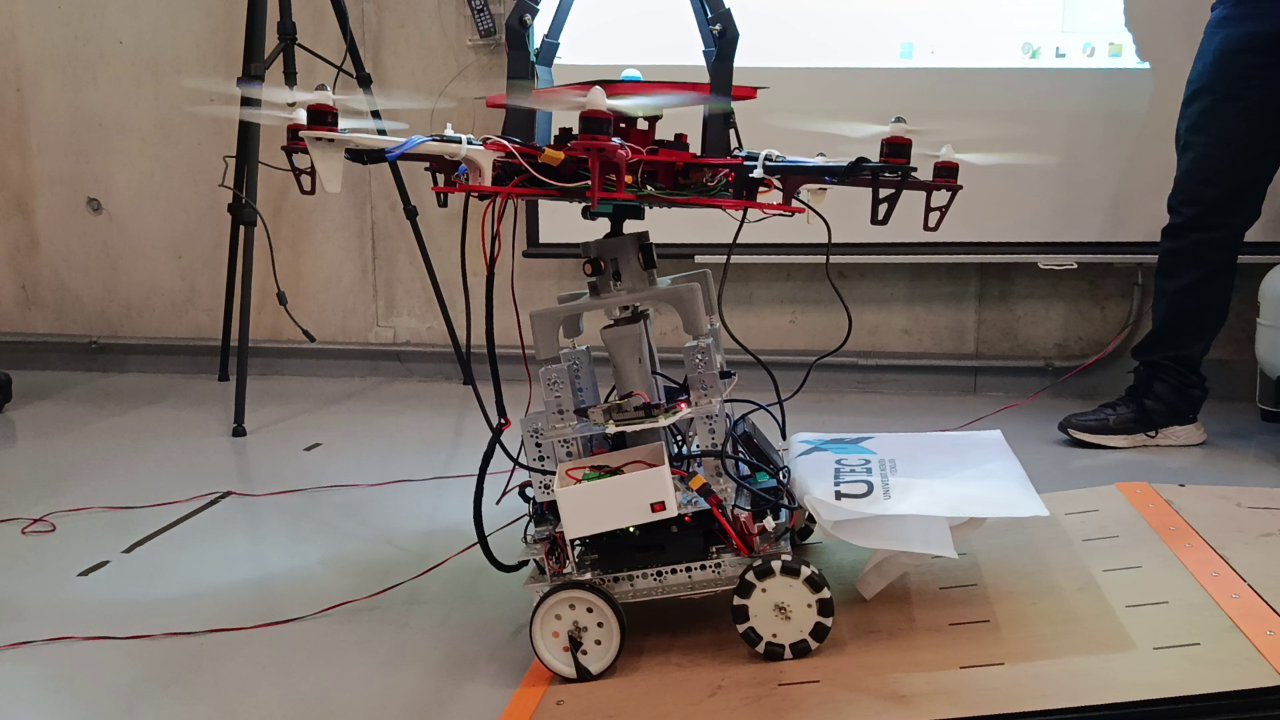
\includegraphics[width=\linewidth]{figures/ensayo23_a.jpg}\caption{BP23-12, 18:55:44.}\end{subfigure}\hfill
  \begin{subfigure}[b]{0.32\textwidth}\centering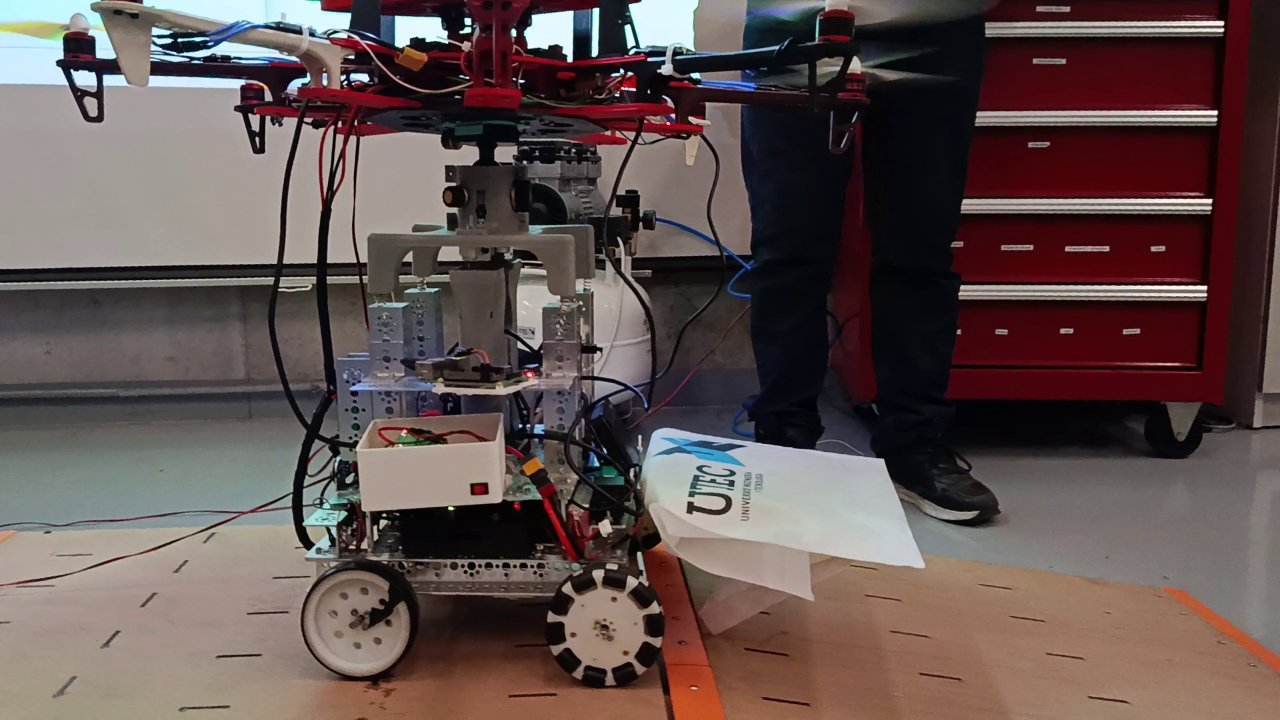
\includegraphics[width=\linewidth]{figures/ensayo23_b.jpg}\caption{BP23-12, 18:55:56.}\end{subfigure}\hfill
  \begin{subfigure}[b]{0.32\textwidth}\centering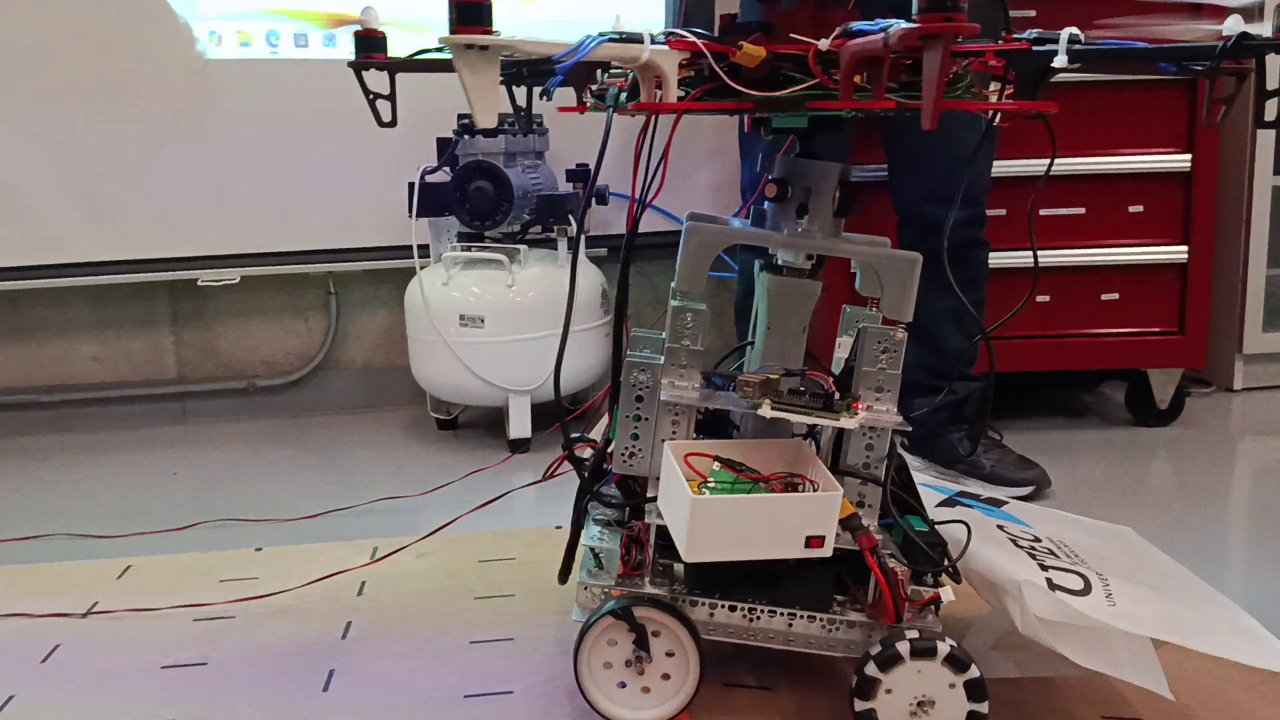
\includegraphics[width=\linewidth]{figures/ensayo23_c.jpg}\caption{BP23-13, 19:01:34.}\end{subfigure}\\[4pt]
  \begin{subfigure}[b]{0.7\textwidth}\centering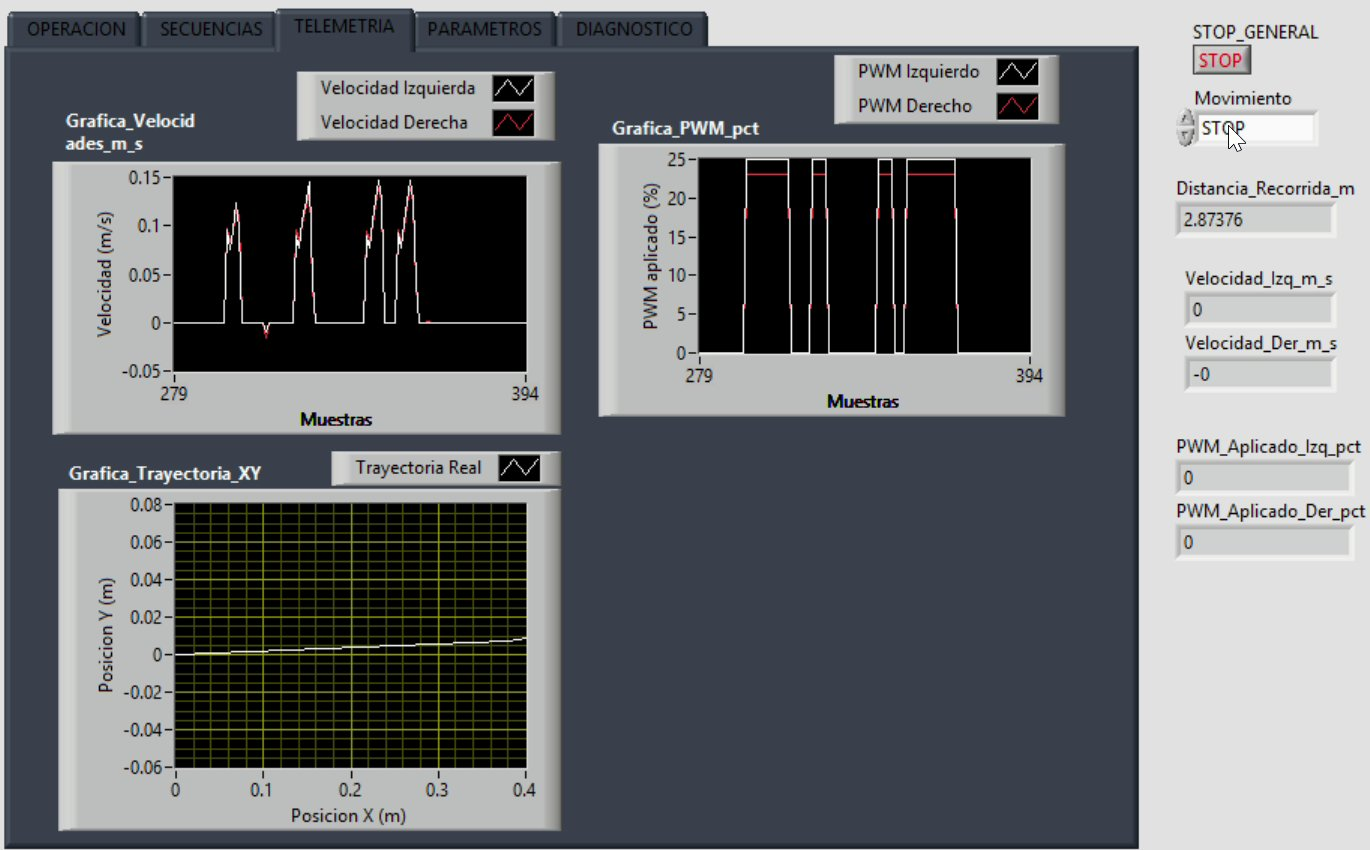
\includegraphics[width=\linewidth]{figures/ensayo23_labview.jpg}\caption{Telemetría de LabVIEW, 18:49:28.}\end{subfigure}
  \caption{Ensayos completos del 23/11. (a)--(c) El robot cruza la rampa con los ocho rotores girando y la bola sobre el plato (videos \texttt{VID\_20261123\_185429} y \texttt{\_190131}). (d) Panel de telemetría de la myRIO en el ensayo BP23-10: velocidad de cada rueda, PWM aplicado (25/23\,\%), trayectoria por odometría y orden \texttt{ADELANTE}.}
  \label{fig:completos23}
\end{figure}

Durante el cruce, la bola estuvo a una mediana de 30--\SI{35}{\milli\metre} del centro y el 80--91\% del tiempo dentro de \SI{50}{\milli\metre}, un error igual o menor que con la base quieta en los mismos ensayos (35--\SI{56}{\milli\metre}) y del mismo orden que los recorridos del 18/11 (mediana de \SI{29.5}{\milli\metre} en la rampa, Tabla~\ref{tab:bp}). La inclinación del dron fue de 0,85--\SI{1.15}{\degree} RMS, con picos de hasta \SI{6.7}{\degree} en los quiebres, y el firmware v11 no cortó los motores en ninguno, a diferencia de los recorridos del 18/11, que terminaron por los cortes de guiñada e inclinación del firmware de banco (Sección~\ref{sec:integrated}). La bola se mantuvo 18--\SI{30}{\second} de cruce en cada ensayo, del orden del cruce completo de la rampa medida (\SI{2.2}{\metre}; el modelo da \SI{19}{\second} con PWM del 25\%, Tabla~\ref{tab:modelval}); los cuatro ensayos terminaron durante el cruce, con la bola saliendo del plato en el tramo final (en BP23-13, al bajar el último quiebre, Fig.~\ref{fig:completos23}c), donde el 18/11 también se concentraban las caídas.

\paragraph{Base: velocidad y rectitud} La telemetría de LabVIEW registró las velocidades de rueda en los recorridos del 23/11. Con PWM del 25\% leyó 0,078--\SI{0.084}{\metre\per\second} en unos tramos y 0,124--\SI{0.134}{\metre\per\second} en otros; el modelo de \eqref{eq:vss} con la masa medida de \SI{10.4}{\kilo\gram} da \SI{0.078}{\metre\per\second} subiendo \SI{10}{\degree} y \SI{0.124}{\metre\per\second} en llano, así que los dos grupos de lecturas coinciden, dentro de un 8\%, con las dos predicciones; la telemetría no indica en qué tramo estaba la base, de modo que la asignación de cada grupo a un tramo es por cercanía. Con PWM del 40\% leyó entre 0,110 y \SI{0.222}{\metre\per\second}; el valor máximo queda un 8--10\% por encima de los \SI{0.201}{\metre\per\second} del modelo en llano. En un recorrido recto de \SI{2.16}{\metre} la odometría terminó con \SI{7.8}{\milli\metre} de desvío lateral (0,4\%) y \SI{-2.7}{\degree} de rumbo, con la compensación de 0,92 en la rueda derecha y el PI de rueda desactivado.

\paragraph{Despegue del dron con la bola encima} En el ensayo BP23-05 se ordenó flotar con la bola en equilibrio (Fig.~\ref{fig:bp23despegue}). El colectivo subió de 1300 a \SI{1750}{\micro\second} en \SI{25}{\second} sin que se perdiera la bola. A las 18:28:04 el módulo despegó en la guía: el láser pasó de 385 a \SI{499}{\milli\metre} (\SI{114}{\milli\metre} de subida) con la inclinación dentro de \SI{2.5}{\degree}, y aterrizó con la orden de aterrizar, sin ningún corte. Es el décimo vuelo en la guía (el primero con el firmware v11) y el primero con el plato y la bola encima. La bola, que medio segundo antes estaba en el centro ($x=\SI{-1}{\milli\metre}$), salió del plato en \SI{0.5}{\second}: el módulo no sube suave sino de golpe, porque la fricción de la guía lo retiene hasta que el empuje la vence, y el acelerómetro registró en ese instante de 0,28 a \SI{1.5}{g}. La aceleración vertical no la puede compensar el plato, así que la corrección está en el despegue: subir más lento cerca del empuje de despegue y enganchar el control de altura en cascada (Sección~\ref{sec:altura}) en cuanto el láser detecta la subida, para que el módulo no siga acelerando hacia arriba.

\begin{figure}[!htbp]
  \centering
  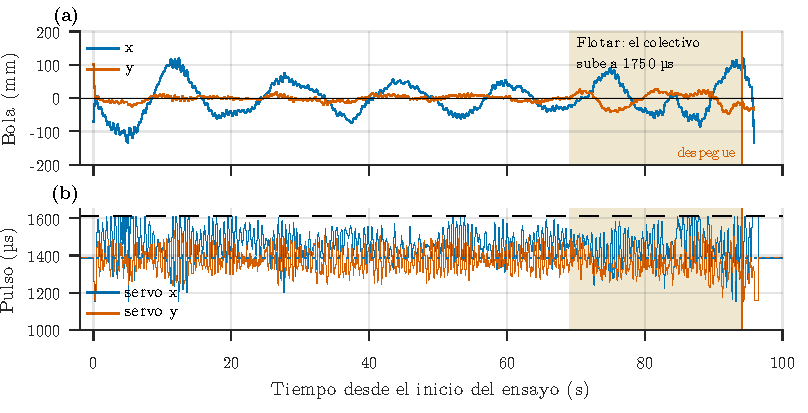
\includegraphics[width=\textwidth]{figures/fig_bp23_despegue.pdf}
  \caption{Ensayo BP23-05 (registro de la Pi a \SI{187}{\hertz}). Arriba: posición de la bola; abajo: pulsos de los servos, con el neutro del eje $x$ (punteado) y su tope (discontinuo). La franja marca la subida del colectivo hasta \SI{1750}{\micro\second} y la línea roja el despegue del dron, cuando la bola sale del plato. Se ve la oscilación lenta en $x$ y el sesgo del servo $x$ por encima de su neutro.}
  \label{fig:bp23despegue}
\end{figure}

\subsection{Base móvil y pruebas integradas}
\label{sec:integrated}
La Fig.~\ref{fig:tests} muestra cuadros de las pruebas integradas. La base, llevando el dron con los rotores girando y la bola sobre el plato, completó:
\begin{itemize}
  \item recorridos rectos y giros en llano;
  \item subidas y bajadas de la rampa de \SI{10}{\degree} en ambos sentidos, repetidas en varias pasadas (videos de las pruebas en la carpeta \texttt{videos/} del repositorio).
\end{itemize}
En los ocho recorridos integrados del 18/11 el dron usó el firmware de banco con el colectivo en \SI{1300}{\micro\second}, es decir, sin descargar peso ($f\approx0$), y los recorridos terminaron así:
\begin{itemize}
  \item cuatro por el corte de guiñada de \SI{20}{\degree}, porque el dron giraba con la base;
  \item tres por el corte de inclinación de \SI{12}{\degree}, medido en 12,0--\SI{12.2}{\degree} con velocidades angulares de hasta \SI{49}{\degree\per\second} al entrar a la rampa, lo que deja solo \SI{2}{\degree} de margen en una pendiente de \SI{10}{\degree};
  \item uno por el operador.
\end{itemize}
Estos eventos confirman el acoplamiento que predice \eqref{eq:pitchlin}: la aceleración de la rótula en los bordes de la rampa actúa sobre el módulo a través del término $-mh_ca_J$, y el modo lento de actitud lo amplifica (Fig.~\ref{fig:transm}b). El enlace UART entre la myRIO y la Pi se implementó en ambos lados y se verificó en la Pi con un puerto serie simulado: las tramas válidas se ejecutaron, las inválidas se rechazaron, se respetó la prioridad de la myRIO y se generó la telemetría de 6 campos. Después se probó con la myRIO conectada (Fig.~\ref{fig:uart}): la Pi envió por la UART la posición de la bola y el VI de la myRIO la recibió y la dibujó en tiempo real en su gráfica $x$--$y$, que recorre todo el plato ($\pm$\SI{150}{\milli\metre}) siguiendo los movimientos de la bola; el indicador de caracteres recibidos se encendió durante la prueba. En esa prueba las gráficas de alabeo y cabeceo del dron quedaron vacías, así que la telemetría del dron hacia la myRIO queda por verificar, y la sesión terminó con el aviso de LabVIEW de conexión perdida con la myRIO.

\begin{figure}[!htbp]
  \centering
  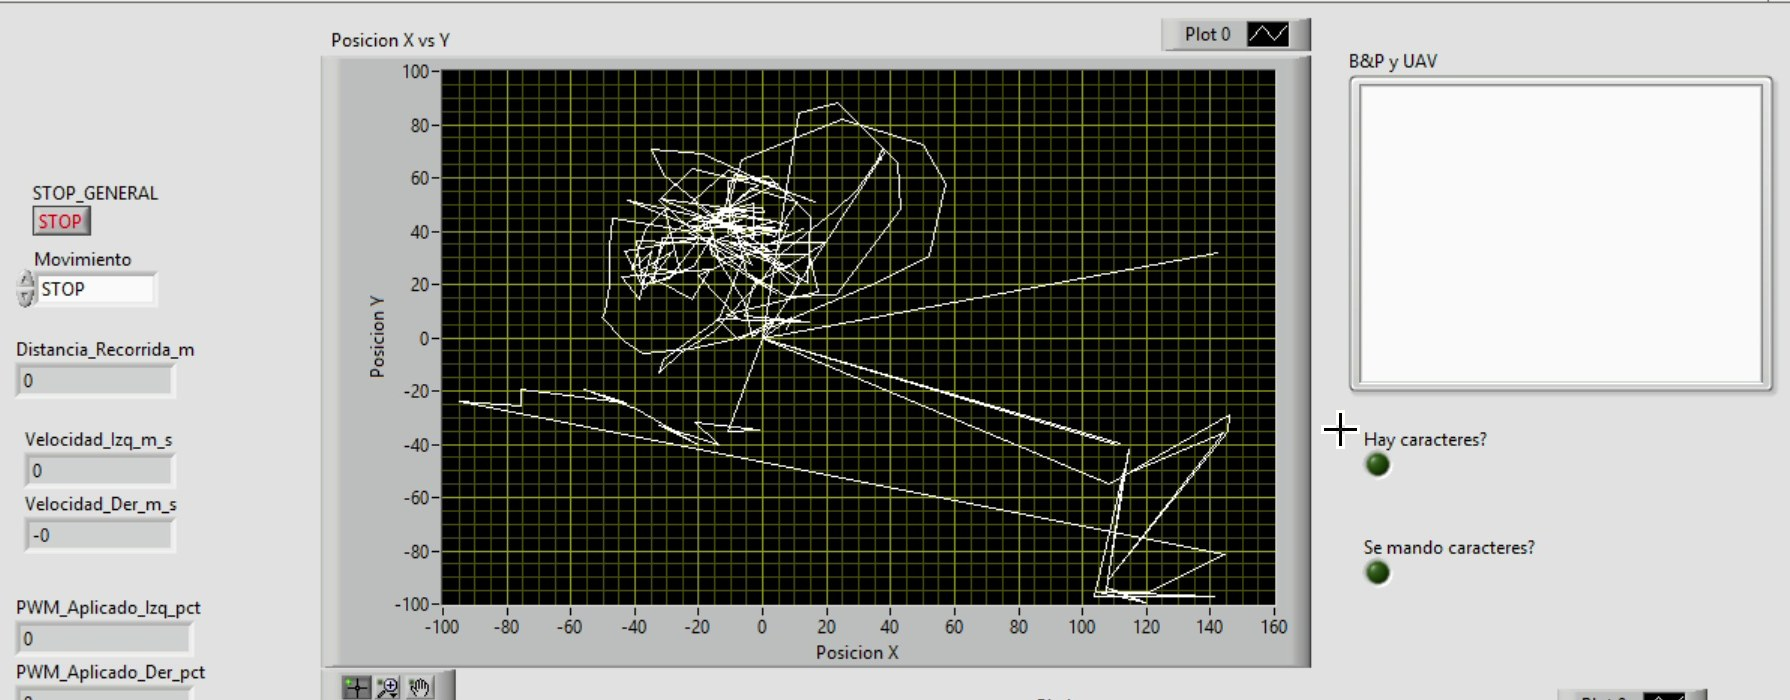
\includegraphics[width=0.9\textwidth]{figures/uart_myrio_bola.jpg}
  \caption{Prueba del enlace UART entre la Raspberry Pi y la myRIO: panel de LabVIEW con la posición de la bola recibida desde la Pi (gráfica $x$--$y$, en mm), la cadena recibida (\texttt{B\&P y UAV}) y los indicadores de recepción y envío.}
  \label{fig:uart}
\end{figure}

%% ---- TODO tras los ensayos finales del 23/11: llenar esta tabla (y descomentarla) ----
% \begin{table}[!htbp]\centering\small
% \caption{Ensayos finales de la base (odometria y video). Error = |posicion final - objetivo|.}
% \begin{tabular}{@{}lrrrr@{}}\toprule
% Ensayo & Objetivo & Medido (media $\pm$ de, $n$) & Error (\%) & Error mediano de la bola (mm) \\\midrule
% Traslacion, llano & 25 cm & & & \\
% Traslacion, llano & 50 cm & & & \\
% Traslacion, 10 grados & 25 cm & & & \\
% Giro sobre el punto medio del eje & 360 grados & & & \\
% Giro sobre una rueda & 360 grados & & & \\
% Subida de 10 grados con modo rampa (f = 0,5) & -- & & & \\
% \bottomrule\end{tabular}\end{table}

\subsection{Validación del modelo}
\label{sec:modelval}
La Tabla~\ref{tab:modelval} compara las predicciones del modelo de la Sección~\ref{sec:model} con las mediciones. Se marcan los parámetros identificados a partir de un conjunto de datos; las comparaciones de las demás filas usan datos que no se emplearon para construir el modelo.

\begin{small}
\setlength{\tabcolsep}{4pt}
\begin{longtable}{@{}>{\raggedright\arraybackslash}p{0.25\textwidth}>{\raggedright\arraybackslash}p{0.22\textwidth}>{\raggedright\arraybackslash}p{0.34\textwidth}>{\raggedright\arraybackslash}p{0.11\textwidth}@{}}
\caption{Predicciones del modelo frente a mediciones.}\label{tab:modelval}\\
\toprule
Magnitud & Modelo & Medición & Ec./Sec. \\
\midrule\endfirsthead
\toprule Magnitud & Modelo & Medición & Ec./Sec. \\ \midrule\endhead
Velocidad de la base, 15\%, llano & \SI{0.072}{\metre\per\second} & 0,06--\SI{0.08}{\metre\per\second} (telemetría de LabVIEW) & \eqref{eq:vss} \\
Velocidad de la base, 15\%, \SI{10}{\degree} & \SI{0.027}{\metre\per\second} & la rampa se subió más lento que el llano (videos) & \eqref{eq:vss} \\
Velocidad de la base, 25\%, llano / \SI{10}{\degree} (23/11) & 0,124 / \SI{0.078}{\metre\per\second} & 0,124--0,134 / 0,078--\SI{0.084}{\metre\per\second} (LabVIEW), error $\le\SI{8}{\percent}$ & \eqref{eq:vss} \\
Velocidad de la base, 40\%, llano (23/11) & \SI{0.201}{\metre\per\second} & máximo 0,217--\SI{0.222}{\metre\per\second} (+8 a +10\%) & \eqref{eq:vss} \\
Colectivo de vuelo estacionario & \SI{1899}{\micro\second} (mapa del firmware); \SI{1770}{\micro\second} (auditoría) & despegue a \SIrange{1725}{1775}{\micro\second} & \ref{sec:ident} \\
Despegue con batería descargada (vuelo 9) & \SI{1787}{\micro\second} (1758--1817) & \SI{1796}{\micro\second} & \eqref{eq:ureq} \\
Despegue con 11,1\,V en reposo & 1850--\SI{2000}{\micro\second}: no flota en régimen sostenido & no flotó & \eqref{eq:ureq} \\
Centro de masa del módulo & $h_c=\SI{0.10}{\metre}$ (CAD) & $h_c=0.14\pm\SI{0.06}{\metre}$, $\delta_x=9.5\pm\SI{1.8}{\milli\metre}$ (identificado) & \eqref{eq:cop} \\
Inclinación recuperable, límites v4--v7 & $\theta^\ast=$ 2,8--\SI{3.8}{\degree} & los vuelos 3--6 derivaron hasta el enclavamiento de \SI{12}{\degree} & \eqref{eq:thetastar} \\
Inclinación recuperable, límites v8--v9 & $\theta^\ast=$ 16--\SI{19}{\degree} & los vuelos 7--9 se mantuvieron 20--\SI{48}{\second} & \eqref{eq:thetastar} \\
Modo lento de actitud en vuelo estacionario & 0,20--\SI{0.30}{\hertz}, $\zeta=$ 0,24--0,42 & picos espectrales en 0,15--\SI{0.23}{\hertz} & \ref{sec:attitude} \\
Lazo de la bola, ganancia derivativa & estable 4,5 e inestable 6 para $K_{b,\mathrm{eff}}=$ 3,5--4,9 & 4,5 estable, 6 inestable (banco) & \ref{sec:ballcontrol} \\
Ganancia de planta de la bola & 6,0 (CAD); 3,5--4,9 (inferida) & 2,5 / 4,9 ($x$/$y$, regresión, $R^2\le0.45$) & \eqref{eq:balltf} \\
Error de la bola debido a la actitud, rotores encendidos & 1,7--\SI{2.1}{\milli\metre} RMS & 16--\SI{21}{\milli\metre} RMS (dominado por $D_b$) & \eqref{eq:propag} \\
Error de la bola, base quieta frente a en movimiento & aumento por las aceleraciones de la base & mediana +9 a \SI{11}{\milli\metre} & \eqref{eq:balllinx} \\
Pendiente de vuelco estático (módulo trabado) & CM del CAD: $x_G=\SI{81}{\milli\metre}$ & \SI{21.5}{\degree} al subir y \SI{30.5}{\degree} al bajar (23/11), es decir $x_G=\SI{88}{\milli\metre}$: el CAD difiere un \SI{8}{\percent} & \eqref{eq:tip} \\
Recorrido de la guía & \SI{77}{\milli\metre} (CAD) & unos \SI{140}{\milli\metre} (medido) & Tabla~\ref{tab:params} \\
Rango de la rótula frente a los quiebres de la rampa & necesario $>\SI{10}{\degree}$ & 35--\SI{53}{\degree} según la dirección & Sec.~\ref{sec:metodologia} \\
Altura con láser calibrado y Kalman & \SI{330}{\milli\metre} (regla) & 317--\SI{334}{\milli\metre} (error $\le\SI{4}{\percent}$) & \eqref{eq:kfz} \\
Control de altura en cascada & 4--\SI{12}{\milli\metre} pico a pico (simulación) & no ensayado en vuelo; el láser con Kalman registró el despegue del vuelo 10 (\SI{114}{\milli\metre} de subida) & \eqref{eq:cascada} \\
Ciclo de rampa (\SI{0.7}{\metre} a \SI{10}{\degree} + \SI{0.8}{\metre} + \SI{0.7}{\metre}), PWM del \SI{15}{\percent} & \SI{41}{\second} en ralentí; \SI{37}{\second} en modo rampa & pendiente (cronómetro) & \eqref{eq:vss}, \eqref{eq:descarga} \\
Cruce de la rampa con PWM del \SI{25}{\percent} (23/11) & \SI{19}{\second} & orden \texttt{ADELANTE} de \SI{25.5}{\second} en BP23-12; bola mantenida 18--\SI{30}{\second} de cruce & \eqref{eq:vss}, \eqref{eq:descarga} \\
\bottomrule
\end{longtable}
\end{small}

El modelo reproduce todas las magnitudes para las que existe una medición, en la mayoría de los casos dentro de la incertidumbre de los parámetros. Su principal discrepancia abierta es el tamaño de la perturbación directa sobre la bola, $D_b$, que el modelo trata como una entrada externa; cuantificar el flujo de los rotores sobre el plato es el siguiente experimento natural. Las predicciones de descarga de peso en la rampa aún no tienen medición.

\subsection{Cumplimiento de los requisitos y limitaciones}
\label{sec:requirements}
\label{sec:limits}
La Tabla~\ref{tab:req} compara los resultados con los escenarios de validación de la guía del curso.

\begin{table}[!htbp]
\centering
\caption{Estado de los escenarios de validación de la guía del proyecto.}
\label{tab:req}
\footnotesize
\renewcommand{\arraystretch}{1.1}
\begin{tabularx}{\textwidth}{@{}>{\raggedright\arraybackslash}p{0.34\textwidth}>{\raggedright\arraybackslash}X>{\raggedright\arraybackslash}p{0.17\textwidth}@{}}
\toprule
Escenario & Evidencia & Estado \\
\midrule
Traslación y giro de la base (llano, \SI{10}{\degree}) & rampa subida y bajada en ambos sentidos; velocidades del 23/11 dentro de un 8--10\% del modelo; desvío lateral del 0,4\% en \SI{2.16}{\metre}; modos de odometría para \SI{25}{\centi\metre}, \SI{50}{\centi\metre} y \SI{360}{\degree} implementados & cumplido en traslación; giro sin métrica final \\
Base en pendiente de \SI{20}{\degree} & no ensayada; sin empuje el vuelco estático medido es \SI{21.5}{\degree} (margen de \SI{0.26}{\metre\per\second\squared} en \SI{20}{\degree}); con el modo rampa ($f=0.35$--0,55) el margen pasa a 0,72--\SI{0.98}{\metre\per\second\squared} (Sección~\ref{sec:porquedron}) & no cumplido; viable con modo rampa, por validar \\
Estimación de la plataforma y de la bola & detección a \SI{187}{fps} en todo el plato; calibración por homografía & cumplido \\
Equilibrio con la base fija & mediana 4,4 / \SI{18.9}{\milli\metre} (dron apagado / encendido, 17/11), sin caídas; 13 tramos continuos de 23--\SI{122}{\second} el 23/11 (\SI{816}{\second}, 10 con rotores), mediana 29--\SI{44}{\milli\metre} (Tabla~\ref{tab:ensayos23}) & cumplido \\
Equilibrio durante la traslación (llano, \SI{10}{\degree}) & mediana 27,9 / \SI{29.5}{\milli\metre} (18/11), P95 por debajo del medio ancho del plato; cuatro ensayos completos del 23/11 cruzando la rampa con los rotores encendidos: mediana 30--\SI{35}{\milli\metre}, 18--\SI{30}{\second} de cruce, sin cortes del dron (Tabla~\ref{tab:completos23}) & cumplido, con caídas en el tramo final de la rampa \\
Equilibrio durante el giro & recorridos con giros incluidos en la condición (c) & cumplido en parte (cortes por guiñada) \\
Etapa intermedia (octocóptero) & RMS en banco $<$\SI{0.4}{\degree}; tres vuelos estacionarios en la guía de \SIrange{20}{48}{\second} (vuelos 7--9); 0,71--\SI{1.0}{\degree} RMS con rotores y la bandeja encima (23/11); despegue y aterrizaje sin corte con la bola encima (vuelo 10, v11) & cumplido en la guía \\
Interfaz y registro & interfaz web, panel de LabVIEW, registros CSV a la tasa de la cámara y del dron & cumplido \\
\bottomrule
\end{tabularx}
\end{table}

Las limitaciones principales son:
\begin{enumerate}[label=(\roman*)]
  \item \textbf{Cortes en los recorridos integrados y funciones pendientes de v11.} En los recorridos del 18/11 el firmware de banco cortó por guiñada (\SI{20}{\degree}) y por inclinación (\SI{12}{\degree}). El firmware v11 resolvió el corte de guiñada en ralentí ($\le\SI{1400}{\micro\second}$) con la ventana deslizante de $\pm\SI{20}{\degree}$ y tope de seguridad de \SI{120}{\degree\per\second}, lo que permitió completar los cuatro cruces de rampa del 23/11 sin cortes. Quedan pendientes escalar el límite de inclinación de \SI{12}{\degree} con la pendiente y validar el seguimiento activo de guiñada (\texttt{yb}) desde la myRIO en giros completos de \SI{360}{\degree}.
  \item \textbf{Batería sin medición.} El firmware no lee la tensión de las LiPo, y el margen de empuje cae con su cuadrado: el vuelo sostenido útil es de 3--\SI{7}{\minute} por par de baterías, y con 11,1\,V en reposo el módulo ya no despega por debajo del límite sostenido (Sección~\ref{sec:bateria}).
  \item \textbf{Ensayos pendientes del protocolo (trabajo futuro).} No se ejecutaron en la campaña del 23/11 la descarga de peso en rampa ($f=0.5$; los recorridos se hicieron en ralentí), el ensayo comparativo D (dron trabado C2 frente a dron libre C3), las repeticiones con cinta de \SI{25}{\centi\metre}, \SI{50}{\centi\metre} y giros de \SI{360}{\degree} (E1), el barrido sinusoidal del plato (E2) ni las pruebas de recuperación desde 2 y \SI{5}{\centi\metre} (E3).
  \item \textbf{Centro de masa y margen de autoridad.} La excentricidad de \SI{9.5}{\milli\metre} exige \SI{0.31}{\newton\metre} permanentes, y la altura del centro de masa sobre la rótula ($h_c\approx\SI{0.14}{\metre}$) hace pequeña la rigidez neta del lazo de actitud (Sección~\ref{sec:attitude}).
  \item \textbf{Mapa de empuje.} El mapa no se identificó con una celda de carga; los datos de despegue indican que $k_F$ es 33--52\% mayor que el supuesto, y su forma con colectivo alto es desconocida.
  \item \textbf{Alimentación.} El BMS original de servos y bobinas falló y en parte de los ensayos se usó una fuente de banco; GPIO5 y GPIO14 emiten pulsos al arrancar el ESP32, lo que obliga a energizar los ESC después del arranque.
  \item \textbf{Visión.} La bola se detecta por color, así que la iluminación debe controlarse.
  \item \textbf{Altura de la rótula.} El centro de masa del módulo está sobre la rótula, así que el módulo es un péndulo invertido ($h_c=0.14\pm\SI{0.06}{\metre}$, polo inestable de \SI{6.1}{\radian\per\second}) y el control de actitud opera cerca del límite por retardo $p\theta_e\approx0.5$. Bajar el centro de masa por debajo de la rótula lo haría pasivamente estable.
  \item \textbf{Parámetros del modelo.} La inercia $\vect J$, la distribución de masas de la base y la resistencia interna de las LiPo son estimaciones basadas en el CAD, en pruebas o en valores típicos, y el retardo del servo se infirió y no se midió; un banco de empuje con celda de carga, un ensayo de péndulo bifilar para la inercia, un ensayo de escalón del servo y una medición de la caída de tensión bajo carga cerrarían estas brechas.
\end{enumerate}
